\documentclass[10pt,a4paper]{article}
\usepackage[utf8]{inputenc}
\usepackage{amsmath}
\usepackage{amsfonts}
\usepackage{amssymb}
\usepackage{dsfont}
\usepackage{graphicx}
\newcommand{\norm}[1]{\left\lVert#1\right\rVert}
\title{cs234 hw2}
\date{2021-12-29}
\author{Jon Sondag}
\setcounter{section}{-1}
\begin{document}
  \maketitle
  \section{Test Environment}
  \subsection{1}
Best path: 0 $\rightarrow$ 2 $\rightarrow$ 1 $\rightarrow$ 2 $\rightarrow$ 1 $\rightarrow$ 0 \\
This path achieves a reward of 4.1.
This is the biggest reward we can achieve because it goes from 2 to 1 as many times as possible.  All other rewards are either smaller by a factor of at least 10, or can't be achieved more often.  Additionally, we get an extra 0.1 for going from state 1 to state 0 from step 4 to 5.

 \section{Q-Learning}
  \subsection{}
  Representing $Q$ in $\Re^{|A|}$ allows us to compute Q-values for all actions with a single forward pass through the network.
  
  \subsection{}
  [coding]
  
  \subsection{}
  From equation (3) in the homework handout, \\
  $L(w) = \mathds{E}\Big [ \big(r + \gamma \max_{a' \in A}(\hat{q}(s',a';\boldsymbol{w}) - \hat{q}(s,a;\boldsymbol{w})\big)^2 \Big ]$ \\
  \\
  Update rule is \\
  $w \leftarrow w + \alpha * -dL/dw$, or \\
  $w \leftarrow w + 2\alpha \big[r + \gamma \max_{a' \in A} \hat{q}(s',a';\boldsymbol{w}) - \hat{q}(s,a;\boldsymbol{w})\big] \nabla_w (-\gamma \max_{a' \in A} \hat{q}(s',a';\boldsymbol{w}) + \hat{q}(s,a;\boldsymbol{w}))$ \\
  
  
  However, the term $-\gamma \max_{a' \in A} q(s',a';w)$ from the update rule above is not included in the update formula in $(2)$.  So the given weight update is $\boldsymbol{not}$ an instance of SGD on the objective $L(w)$.
  
  \subsection{}
  Update rule is \\
  $w \leftarrow w + \alpha * -dL/dw$, or \\
  $w \leftarrow w + 2\alpha \big[r + \gamma \max_{a' \in A} \hat{q}(s',a';\boldsymbol{w}) - \hat{q}(s,a;\boldsymbol{w})\big] \nabla_w ( \hat{q}(s,a;\boldsymbol{w}))$ \\
  
  Yes, the given weight update is an instance of SGD (within a factor of 2).

  \subsection{}
  The tradeoff is: \\
  For C large, the update rule is an instance of SGD. \\
  For C small, the update rule is updated more frequently, and in a sense better tracks our training data.

  \subsection{}
  The dataset $\mathcal{D}$ differs from the replay buffer $\mathcal{D}$ as follows: \\
  \begin{itemize}
  \item The dataset uses each s,a,r,s' sample only once, whereas the replay buffer will use each sample potentially many (or zero) times.
  \item Additionally (importantly for SGD) the training samples we select from the replay buffer are drawn at random, breaking up potential correlations between consecutive data points.
  \end{itemize}
  
  \section{Linear Approximation}
  
  \subsection{}
  If $w \in \mathbb{R}^{|S||A|}$ \\
  and \\
  $[\delta(s,a)]_{s',a'}=\begin{cases}
  1, & \text{if}\ s'=s, a'=a \\
  0, & \text{otherwise}
  \end{cases}$ \\
  and \\
  $\hat{q}(s,a,w)=\boldsymbol{w}^T\delta(s,a)$ \\
  then \\
  $[\hat{q}(s,a,w)]_{s',a'}=\boldsymbol{w}[s',a']$ (using $s'$ and $a'$ to index into $\boldsymbol{w}$) \\
  This is the same as the tabular case, with the matrix $\boldsymbol{w}$ taking the place of the tabular matrix $Q$.
  
  \subsection{}
  The update for $\boldsymbol{w}$ is: \\
  $w \leftarrow w + \alpha(r + \gamma\max_{a'\in{A}}\boldsymbol{w}[s',a']-\boldsymbol{w}[s,a])$, the same as the update given in equation (1) in the homework handout.
  
  \subsection{}
  [coding]
  
  \subsection{}
  Yes, an optimal reward of 4.1 is achieved on the test environment. Plot: \\
  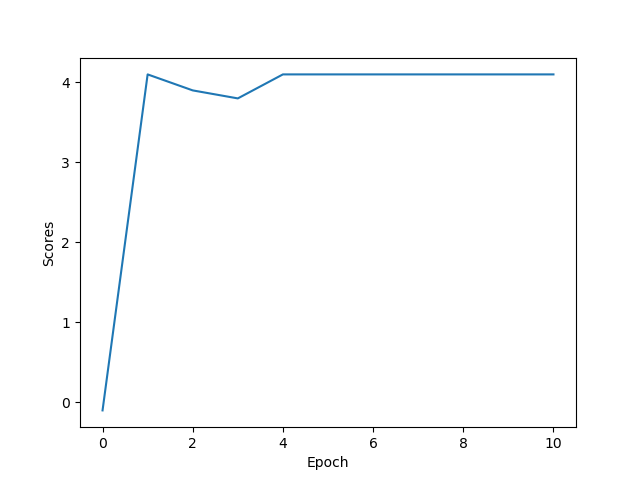
\includegraphics[scale=0.5]{scores_q2_linear.png}
  
  \section{Implementing DeepMind's DQN}
  
  \subsection{}
  [coding]
  
  \subsection{}
  The model takes more epochs to converge, but training the DQN is actually slightly faster than the linear model.  Plot: \\
  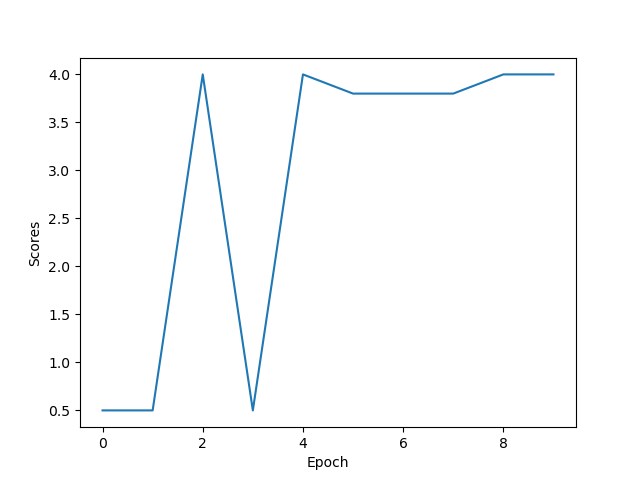
\includegraphics[scale=0.5]{scores_q3_nature.png}  
  
  \section{DQN on Atari}
  
  \subsection{}
  The agent shows some small signs of improvement at the very beginning of training but then avg reward, max reward, loss, etc all flattened out after ~150k steps out of the 500k were complete.  I don't think that training for a larger number of steps would likely yield further improvements in performance as these metrics have stopped improving. \\
  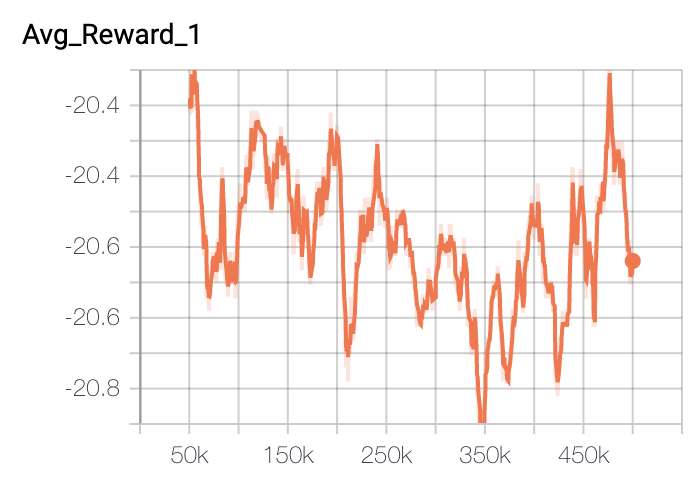
\includegraphics[scale=0.5]{q4_avg_reward.png}
  
  \subsection{}
  I was able to get a score of approximately $-2$ after 5 million steps, lower than the expected score of 13-15.  Running for more than 5 million steps may have helped as the score was still improving when training was terminated.  \\
  Training was run using the network architecture from both \\ $\emph{Playing Atari with Deep Reinforcement Learning}$ and \\
  $\emph{Human-level control through deep reinforcement learning}$, 
  (see get\_q\_values\_op in q3\_nature.py) and the best results are in this plot: \\
  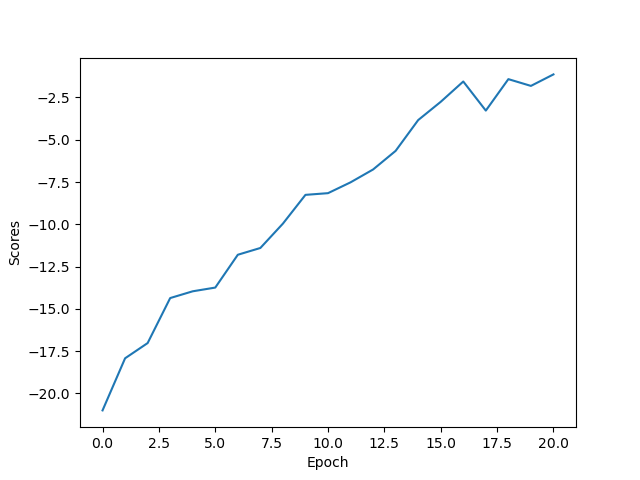
\includegraphics[scale=0.5]{scores_q5_atari_nature.png}

  \section{\emph{n}-step Estimators}
  
  n-step SARSA target: 
  $r_t + \gamma r_{t+1}+...+\gamma^n\hat{q}(s_{t+n}, a_{t+n})$ \\
  Estimator based on n-step SARSA target: \\
  $\hat{q}(s, a) = \mathds{E}\big[r_t + \gamma r_{t+1}+...+\gamma^n\hat{q}(s_{t+n}, a_{t+n})\big | s_t=s,a_t=a,\pi]$ \\
  Split this into two parts: \\
  $\hat{q}_0^{n-1}(s,a)= \mathds{E}\big[r_t + \gamma r_{t+1}+...+\gamma^{n-1}r_{t+n-1}\big | s_t=s,a_t=a,\pi]$ \\
  $\hat{q}_n^{\infty}(s, a) = \mathds{E}\big[\gamma^n\hat{q}(s_{t+n}, a_{t+n})\big | s_t=s,a_t=a,\pi]$ \\
  \\
  Then $Bias(\hat{q}(s,a)) \leq Bias(\hat{q}_0^{n-1}(s,a)) + Bias(\hat{q}_n^{\infty}(s,a))$ \\
  Since $\mathds{E}(|X_1+X_2|) \leq \mathds{E}(|X_1|+|X_2|)$ \\
  \\
  $Bias(\hat{q}_0^{n-1}(s,a))=0$ since by definition \\
  $\mathds{E}[\hat{q}_0^{n-1}]-\mathds{E}\big[r_t + \gamma r_{t+1}+...+\gamma^{n-1}r_{t+n-1}\big] = 0$ \\
  \\
  $Bias(\hat{q}_n^{\infty}(s,a))$ \\
  $= \sum_{\forall a, \forall s}\big[p(a_{t+n}{=}a',s_{t+n}{=}s'|a_t{=}a,s_t{=}s)[\gamma^n\hat{q}(s',a')-\mathds{E}(\gamma^nr_{t+n}+\gamma^{n+1}r_{t+n+1}+...|s_{t+n}{=}s',a_{t+n}{=}a')\big]$ \\
  $ = \gamma^n\sum_{\forall a, \forall s}\big[p(a_{t+n}{=}a',s_{t+n}{=}s'|a_t{=}a,s_t{=}s)[\hat{q}(s',a')-\mathds{E}(r_{t+n}+\gamma r_{t+n+1}+...|s_{t+n}{=}s',a_{t+n}{=}a')\big]$
  $ = \gamma^nBias(\hat{q}(s,a))$, because $Bias(\hat{q}(s,a))=Bias(\hat{q}(s',a')), \forall a, \forall s$ and  the horizon is infinite \\
  \\
  Then since $\gamma^n < 1$ the n-step SARSA is less biased.
  
  

\end{document}